% !TeX root = ../../thesis.tex
\chapter{Large-scale phylodynamics of HBV across millennia}\label{ch:chapter3}

\begin{minipage}[b]{0.6\textwidth}
    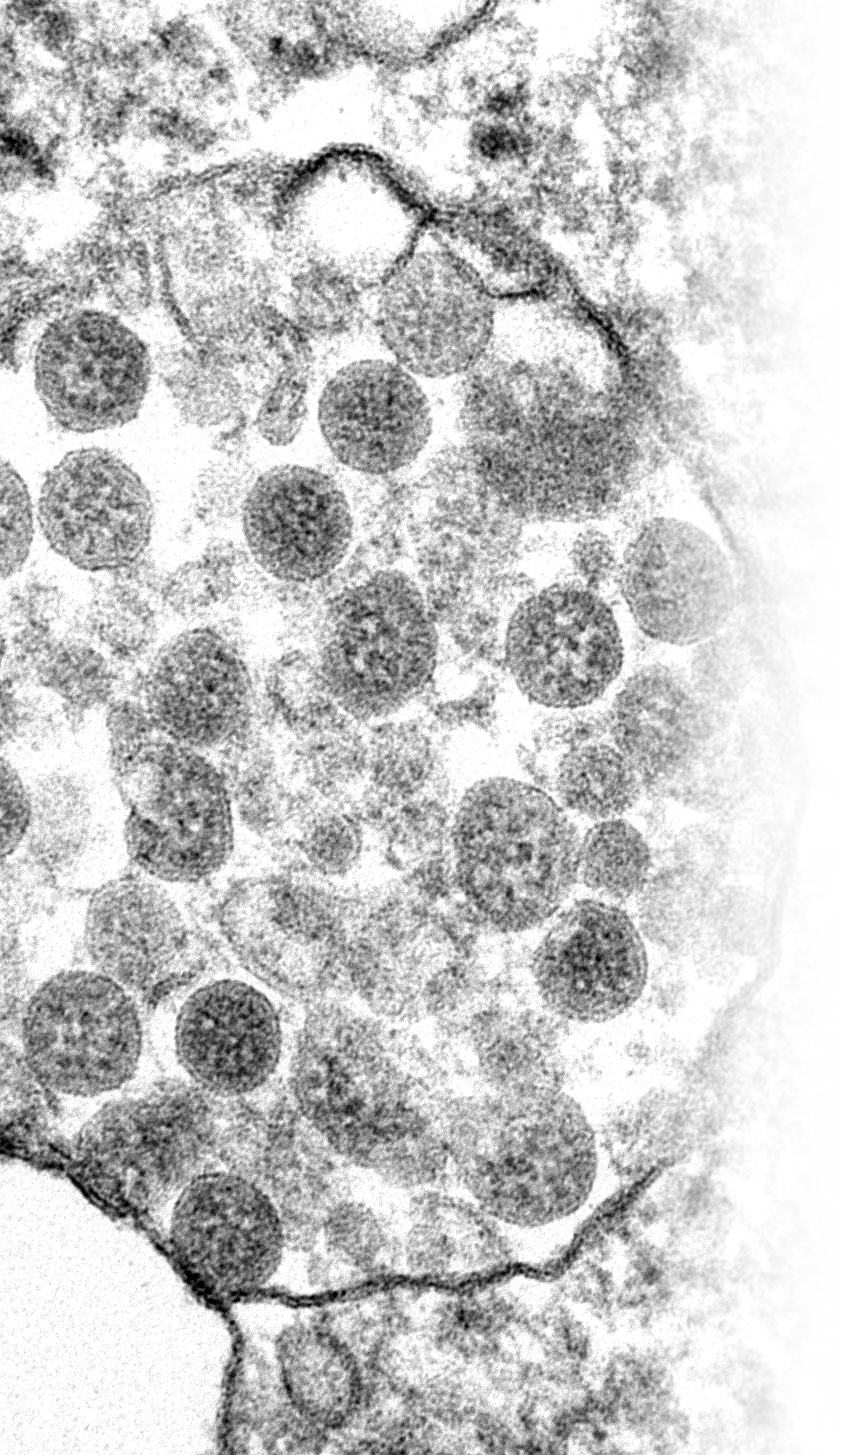
\includegraphics[height=11cm]{title2} % Note: image needs to be cropped and faded
    % https://phil.cdc.gov/Details.aspx?pid=23312
  \end{minipage}
  \hfill
  \begin{minipage}[b]{0.35\textwidth}
    \footnotesize
    \begin{flushright}
      \textit{``Age and treachery\\always overcome\\youth and enthusiasm.''} \\
      --- David Potter, \\my entire childhood
    \end{flushright}
    \vspace{2cm}
  \end{minipage}

\clearpage

% I chose Chicago format for this citation, but I need to check 
% if KUL has specific requirements

\singlespacing

\hrule
\vspace*{12pt}
This chapter was published as \textbf{Barney I. Potter, Marijn Thijssen, Nídia Sequeira Trovão, Andrea Pineda-Peña, Marijke Reynders, Thomas Mina, Carolina Alvarez et al.} "Contemporary and historical human migration patterns shape hepatitis B virus diversity." \textit{Virus Evolution} 10, no. 1 (2024): veae009.
I performed phylogenetic and phylogeographic analysis and wrote the manuscript.
Other authors contributed to the study design, data collection, and manuscript editing.

This version contains some small changes (mostly related to wording) at the suggestion of thesis readers. Those changes do not change any of the results or implications of this study.
\vspace*{12pt}
\hrule

\onehalfspacing

\section{Abstract}
Infection by hepatitis B virus (\gls{hbv}) is responsible for approximately 296 million chronic cases of hepatitis B, and roughly 880\,000 deaths annually.
The global burden of \gls{hbv} is distributed unevenly, largely owing to the heterogeneous geographic distribution of its subtypes, each of which demonstrates different severity and responsiveness to antiviral therapy.
It is therefore crucial to the global public health response to \gls{hbv} that the spatiotemporal spread of each genotype is well characterized.
In this study, we describe a collection of 133 newly-sequenced \gls{hbv} strains from recent African immigrants upon their arrival in Belgium.
We incorporate these sequences---all of which we determine to come from genotypes A, D, and E---into a large-scale phylogeographic study with genomes sampled across the globe.
We focus on investigating the spatio-temporal processes shaping the evolutionary history of the three genotypes we observe.
We incorporate several recently published ancient \gls{hbv} genomes for genotypes A and D to aid our analysis.
We show that different spatio-temporal processes underlie the A, D and E genotypes, with the former two having originated in southeastern Asia, after which they spread across the world.
The \gls{hbv} E genotype is estimated to have originated in Africa, after which it spread to Europe and the Americas.
Our results highlight the use of phylogeographic reconstruction as a tool to understand the recent spatiotemporal dynamics of \gls{hbv}, and highlight the importance of supporting vulnerable populations in accordance with the needs presented by specific \gls{hbv}genotypes.


\section{Introduction}
Hepatitis B virus (\gls{hbv}) imposes a significant global burden to public health \citep{pourkarim2011molecular,malik2022viral}, causing about 880\,000 deaths per year \citep{revill2020evolution} despite over two decades of efforts by the global community under the banner of the World Health Organization \citep{pourkarim2018irans}.
The efficient implementation of prevention and control measures to combat the spread of \gls{hbv} requires detailed insight into the epidemiology of the separate lineages circulating in a given region \citep{schweitzer2015estimations,pourkarim2011guidelines}.
Such information at both country and continent levels is pivotal for implementing effective intervention strategies and estimating the burden of disease accurately \citep{pourkarim2011molecular}.
Both effective antiviral therapies and a widely available vaccine have contributed to significant decreases in the risk of \gls{hbv} infection globally \citep{lu2020virus-like}, however their effectiveness can vary significantly by \gls{hbv} genotype \citep{bottecchia2011detection}.

The global genetic diversity of \gls{hbv} is classified into eight approved genotypes (A--H) and two tentative genotypes (I and J).
These genotypes are further subdivided into more than 45 subgenotypes and quasi-subgenotypes \citep{pourkarim2014molecularidentification,thijssen2020novel}.
Increasing evidence suggests that its genotypes and subgenotypes are determinants for patients' disease progression and may prompt heterogeneous responses to antiviral therapy \citep{mcmahon2009influence,croagh2015genotypes,shen2014hepatitis,pourkarim2014molecularcharacterization,zhang2020rapidly,mina2015genomic}.
The genotypes and subgenotypes of \gls{hbv} show distinct geographical distributions.
For example, genotype A (\gls{hbv}-A) subgenotype A2 is dominant in Europe, whereas subgenotype A1 is mostly prevalent in Africa and East Asia.
Genotypes B and C circulate with high frequency in Southeast Asia and the Pacific Islands \citep{norder2004genetic}.
While genotype D (\gls{hbv}-D) is distributed worldwide, subgenotype D1 is the most prevalent \gls{hbv} subgenotype in western Asia and the Mediterranean Basin \citep{zehender2012spatial,al-qahtani2020molecular,trovao2022reconstruction}, and subgenotypes D2 and D3 are prevalent in eastern Europe \citep{pourkarim2014molecularidentification,pineda-pena2015epidemiological}.
Genotype E (\gls{hbv}-E) is mainly prevalent in West Africa \citep{ingasia2020global}, whereas genotype F is one of the most prevalent genotypes circulating in South and Central America \citep{pujol2020hepatitis}.
Genotype G is a rarely isolated genotype in France, the United States, and Belgium \citep{kay2007hepatitis,mina2015genomic}.
Genotype H has been occasionally reported in Japan but is commonly encountered in Central and South America.
Additionally, two new tentative genotypes (I and J) have been proposed, which are most likely recombinant strains of the previously identified genotypes \citep{pourkarim2014molecularidentification}.

The global epidemiology of \gls{hbv} infection is characterized by hepatitis B surface Antigen (\gls{hbsag}) seroprevalence, which displays strong geographical variation.
Regions may be classified as low seroprevalence (seroprevalence $< 2\%$), such as European countries, intermediate seroprevalence ($2\%$ to $7\%$; e.g. Alaska, the Mediterranean basin, and India), or high seroprevalence (seroprevalence $> 8\%$), such as the South Pacific and countries of Sub-Saharan Africa.
In high seroprevalence regions, \gls{hbv} is considered to be endemic.
Viral transmission routes largely depend on regional prevalence \citep{pourkarim2011molecular}.
A study by the WHO in 2015 showed that global migration trends are crucial to the disease burden and gradual increase of the chronic reservoir in industrialized, low-endemicity countries receiving new waves of migrants from high- and intermediate-endemicity countries without obligatory vaccination \citep{sharma2015immigration}.
Consequently, large migration events have a considerable impact on the prevalence of communicable and contagious diseases like \gls{hbv}, since there are significant differences of \gls{hbv} prevalence in ``source'' and ``sink'' populations \citep{chu2013changing}.
It has been frequently reported that non-endemic \gls{hbv} strains carried by streams of immigrants are changing the viral epidemiological profile in the destination countries \citep{pourkarim2011molecular,chu2013changing,khan2008transmission,mina201715,coppola2017hepatitis,thijssen2019mass}.
Besides their different geographical distribution, genotypes of \gls{hbv} possess genotype-specific mutations in their open reading frames (\gls{orf}s).
The introduction of these strains into countries where prophylaxis, diagnostic, and therapeutic protocols have been implemented based on native \gls{hbv} strains could potentially raise serious concerns \citep{lampertico2015optimal,velkov2020global,limeres2019impact}.
Furthermore, mutations associated with antiviral resistance have been reported in \gls{hbv} strains sequenced from patients who had recently migrated into Europe, even before exposure to treatment \citep{bottecchia2011detection,selabe2007mutations}.
European countries are now faced with new public health challenges to control \gls{hbv} incidence and prevalence, necessitating updated policies for screening, monitoring, and preventing transmission from large reservoirs \citep{schweitzer2015estimations,thijssen2019mass}.

Historically, Belgium has witnessed high rates of immigration, particularly from African countries, with intermediate to high \gls{hbv} seroprevalence \citep{schweitzer2015estimations}.
However, until now there has been a dearth of comprehensive evolutionary analyses of non-domestic \gls{hbv} strains in Belgium.
In this study, we describe a collection of \gls{hbv} strains isolated from patients who had recently immigrated to Belgium from a number of African countries.
Many of the viruses may potentially carry medically important genomic mutations, complicating public health interventions.
Due to the limited global epidemiological insights and the potential impact of continued spread of such strains, we here conduct a molecular epidemiological study investigating the spatio-temporal processes shaping the \gls{hbv} genotypes imported to Belgium, as well as their clinical characterization in a sample collection spanning half a decade.
Our analyses differ from other recent studies such as that performed by \citet{kocher2021ten} in that we analyze each genotype independently in order to understand the spatiotemporal factors that have contributed to the global proliferation of each genotype.


\section{Materials and Methods}
\subsection{Study population \& supplemental sequence selection}
One hundred and thirty-three surface antigen (\gls{hbsag}) positive individuals, who immigrated to Belgium from Africa between 2005 and 2010 were enrolled in this study.
Serum samples were collected from patients upon their first clinical visit during the study.
Virological and serological markers were assayed, and demographic information like sex, age, origin, possible transmission routes and antiviral therapy were collected.
For our analyses, we supplemented these novel sequences with all \gls{hbv}-A, \gls{hbv}-D and \gls{hbv}-E sequences available from the NCBI genome database \citep{sayers2022database} during our study period.
Supplemental sequences from NCBI were screened for quality and excluded if they showed signatures of recombination or gaps longer than 50bp in length.
This study was approved by the Ethical Committee of University hospital of KU Leuven (S56121/ML10229).

\subsection{Extraction, amplification, \& complete genome sequencing}
Viral DNA was extracted from sera using the QIAmp1 Viral DNA mini kit (Qiagen, Hilden, Germany).
Complete \gls{hbv} genomes were amplified and sequenced using a previously described method \citep{pourkarim2011molecular,pourkarim2009phylogenetic}.
To eliminate any recombinant isolates that may influence the topology of phylogenetic trees of \gls{hbv}, we screened for recombination events among our newly sequenced strains and strains retrieved from the database using the \gls{hbv} NCBI genotyping tool (https://www.ncbi.nlm.nih.gov/projects/genotyping/formpage.cgi).
This tool provides an estimation of recombination signatures along with the full-length sequences of \gls{hbv} strains.
If there was any indication of hybrid genomes, further investigation was conducted using SimPlot software, version 3.5.1, and bootScan \citep{lole1999full-length}.
Detected recombinant strains were then confirmed through the construction of phylogenetic trees using different targeted segments.

\subsection{Genotyping \& subgenotyping}
We performed whole-genome alignment using MAFFT v7.0 \citep{katoh2013mafft}, and used the same genome alignments for subsequent analyses.
In order to determine genotype and subgenotype of sequenced strains, maximum-likelihood phylogenetic trees were constructed using IQ-TREE v1.6.12 \citep{nguyen2015iq} under an \gls{hky} nucleotide substitution model \citep{hasegawa1985dating}, accommodating among-site rate heterogeneity through a discretized gamma distribution \citep{yang1994maximum}.
Clade support was verified using UFBoot2 with 1\,000 replicates \citep{hoang2018ufboot2}.
We assigned new sequences genotype and subgenotype designations based on their phylogenetic placement.

\subsection{HBV Mutational Patterns}
Newly sequenced \gls{hbv} full-length genomes are genotyped through phylogenetic analysis before mutational analysis.
Subsequently, the different open reading frames (\gls{orf}s) of these strains are aligned with corresponding \gls{orf}s of reference genomes (the same genotype and subgenotype) at the nucleotide or protein level.
Reference strains retrieved from GenBank are typically associated with papers that present correlations between mutations and conditions such as phenotypically or genotypically antiviral resistance, vaccine or diagnostic escape strains in vivo and in vitro.
These mutations are considered as ``medically important mutations'' in the literature.
Needless to say, in the assessment of \gls{hbv} mutational patterns, variations at the nucleotide level are studied in the \textit{precore}, \textit{core} and \textit{X} genes, while mutations related to the \textit{pol} gene and \textit{S} gene are identified at the protein level.

\subsection{Bayesian phylogenetic inference}
We started by investigating the temporal signal of each genotype using TempEst \citep{rambaut2016exploring}.
We first estimated an unrooted phylogeny for each genotype using maximum-likelihood inference produced in the previous step.
Sequences that showed incongruent temporal patterns were excluded from further analyses.
Because of spatial heterogeneity and clinical differences exhibited by each of \gls{hbv}'s genotypes, we chose to analyze each genotype independently.
This allowed us to not only more specificially characterize the spatiotemporal dynamics of each genotype of interest independently, but also split the computational load between three separate analyses, affording greater scale in each individual analysis.
This resulted in a dataset with 583 \gls{hbv}-A sequences (dated 1979--2014), 764 \gls{hbv}-D sequences (dated 1975--2012), and 234 \gls{hbv}-E sequences (dated 1994--2010).
Phylogenetic relationships were inferred for each of the datasets separately by performing Bayesian phylogenetic inference using Markov chain Monte Carlo (\gls{mcmc}), as available via the BEAST v1.10 package \citep{suchard2018bayesian}.
We used an uncorrelated relaxed molecular clock with branch rates drawn from an underlying lognormal distribution to account for evolutionary rate variation among lineages, with a constant demographic model as the tree prior \citep{kingman1982coalescent,drummond2002estimating}.
To accommodate the impact of the overlapping regions in the \gls{hbv} genome on the substitution process of each codon position, we assumed an \gls{hky} substitution model \citep{hasegawa1985dating} without codon partitioning, with among-site rate heterogeneity through a discretized gamma distribution \citep{yang1994maximum}.
We performed at least three independent replicates of our \gls{mcmc} analysis to ensure proper convergence, with each replicate having a different starting seed to achieve proper statistical mixing and running for at least 500 million iterations to achieve convergence.
Chains were sampled every 10,000 iterations, and we combined all replicates to form a single posterior distribution.
We assumed default priors for all other parameters in BEAST for these analyses and used the BEAGLE v3 \citep{suchard2009many-core,ayres2019beagle} high-performance computational library to speed up the likelihood calculations.
All relevant parameters exhibited proper statistical mixing, reporting ESS values over 200 as assessed using Tracer v.1.7 \citep{rambaut2018posterior}, with statistical uncertainty reflected by the 95\% highest posterior density (HPD) interval.

Following the analysis of the contemporary genomic data sets, and to ensure sufficient temporal signal in the data, we repeated the analysis of \gls{hbv}-A and \gls{hbv}-D using available ancient genomes, collected from mummified tissue ranging in age from 450 years old to $\approx4,200$ years old and spanning from Italy, across Eastern Europe, and into Central Asia \citep{ross2018paradox,muhlemann2018ancient}.
This resulted in the addition of four ancient genomes to the \gls{hbv}-A dataset and five ancient genomes to the \gls{hbv}-D dataset.
No ancient sequences were available to add to the \gls{hbv}-E dataset.
Phylogenetic inference was performed under the same model parameters as analyses without ancient genomes, but used an updated lognormal evolutionary rate prior ($\mu=-11.3474$, $\sigma=1.22$) derived from the \gls{hbv} evolutionary rate estimated by Muhlemann et al. (2018) of $1.18 \times 10^{-5}$ substitutions per site per year, based on the inclusion of ancient sequences.
Default priors were used for all other parameters.
For each subtype, \gls{mcmc} chains were run for 500 million iterations and were sampled every 25\,000th iteration.
Three replicates of each subtype were run using different starting seeds to ensure proper convergence and statistical mixing.
A single combined posterior distribution was formed by combining all replicates for each subtype, removing an appropriate proportion of each chain as burn-in
Maximum clade credibility (\gls{mcc}) trees were summarized using TreeAnnotator v1.10 \citep{suchard2018bayesian} and the resulting trees were visualized in FigTree v1.4.3 and baltic v.0.1.5 (https://github.com/evogytis/baltic accessed on 10 June 2020).

\subsection{Phylogeographic inference}
From the combined posterior distribution of each genotype's phylogenetic reconstruction, 1,000 trees were sampled and used to perform subsequent Bayesian phylogeographic reconstruction in \gls{beast} using empirical tree distributions \citep{pagel2004bayesian}.

This analysis modeled geographic locations as discrete traits, and allowed for different migration rates to and from each location \citep{lemey2009bayesian}.
This approach conditions on the geographic locations recorded at the tips of the trees and models the transition history among those locations as a time-reversible continuous-time Markov chain (\gls{ctmc}) process to infer the unobserved locations at the internal nodes of each tree.
\gls{beast} default priors were used for each parameter.
For these reconstructions, \gls{mcmc} chains were run for 10 million iterations and sampled every 10,000th iteration.
The links between locations that contribute significantly to explaining the migration history were identified using a Bayesian stochastic search variable selection (\gls{bssvs}) procedure \citep{lemey2009bayesian}, and SpreaD3 \citep{bielejec2016spread3} was used to calculate the Bayes factor (\gls{bf}) support for these links.
We quantify geographic transitions by logging Markov jumps and rewards through the phylogeographic analysis.
We note that the data consist of a heterogeneous number of sequences for each location (Suppl.~Tables~\ref{suptab:hbv-s1},~\ref{suptab:hbv-s2},~\ref{suptab:hbv-s3}) which show strong sampling bias between individual countries that can strongly impact the outcome of a discrete phylogeography study \citep{maio2015new}.
To mitigate this issue, we opted to group sequences into continental regions, aiming to contain a number of sequences of the same order of magnitude where possible: Africa, the Americas, East \& South Asia, Europe, and West \& Central Asia.
We note that for \gls{hbv}-E, no samples from East \& South Asia nor West \& Central Asia were available.

\subsection{Statistical analysis}
Statistical analyses were performed using Stata software version 16.1 for Windows.
Categorical variables are expressed as frequencies; continuous variables are expressed as either means and standard deviations or medians and interquartile ranges, according to their distributions.
Chi-squared test and Fisher's exact test were applied to assess the association between categorical variables.
T-test and Mann-Whitney-Wilcoxon test were used to assess continuous variables.
The significance level was set to 0.05.


\section{Results}
\subsection{Lineages circulating in Belgium and new isolates}
We originally investigated 133 individuals coming from 15 countries in Sub-Saharan Africa between 2005 and 2010.
The majority are originally from the Republic of the Congo ($n=44$; $33\%$), Rwanda ($n=23$; $17.25\%$) and Guinea (n=21; 15.75\%).
The country of origin for one individual was unknown.
Most of the individuals were male ($n=96$; $72\%$) and the median age was 30 years [interquartile range (IQR) $= 25$--$37$].
Nineteen individuals ($14\%$) were co-infected with human immunodeficiency virus (\gls{hiv}), while three ($2\%$) were hepatitis C virus (\gls{hcv}) carriers.
Positive e-antigen (eAg) was present in 78 cases ($58.65\%$) (Suppl.~Table~\ref{suptab:hbv-s1}).
No significant differences were observed between \gls{hbv}/\gls{hiv} co-infected patients and \gls{hbv} mono-infected patients in different genotype groups, in terms of medically important mutations at different strain \gls{orf}s.

Phylogenetic analysis and nucleotide divergence analysis of sequences with full-length genomes ($n=121$) and large S genes ($n=12$) revealed three distinct \gls{hbv} genotypes circulating in African immigrants in Belgium.
The most frequently identified genotypes were \gls{hbv}-E ($n=67$, $50.4\%$) and \gls{hbv}-A ($n=55$, $41.4\%$), with the remaining sequences ($n=11$, $8.3\%$) belonging to HBV-D.
Recombination was explored using SimPlot and BootScan (Suppl.~Table~\ref{suptab:hbv-s2} and Suppl.~Fig.~\ref{supfig:hbv-s1}).
The genomes of three isolates (ID: MB-58, MB-56 and MB-92), from one patient of Guinea and two patients of Rwanda, showed recombination: between \gls{hbv}-A and \gls{hbv}-E in MB-58, and between \gls{hbv}-D and \gls{hbv}-E in both MB-56 and MB-92 (Suppl.~Fig~\ref{supfig:hbv-s1}).
MB-58 harbors 900 base pairs (bp) of \gls{hbv}-E (1100--2000 bp) on a backbone of \gls{hbv}-A.
MB-92 carries 600 bp (1800--2400 bp) of \gls{hbv}-E within \gls{hbv}-D, with the wild type length of 3182 bp.
However, MB-56 harbors the same piece of \gls{hbv}-E on a backbone of \gls{hbv}-D with 3212 bp of wild type genome length of \gls{hbv}-E.

\subsection{HBV Mutational Patterns}
For our new sequences, single nucleotide polymorphisms and amino acid polymorphisms were assessed throughout the genome.
We further evaluated if the genotypes identified were associated with the presence of specific drug resistance mutations in the \textit{pol} gene and medically important mutations at \textit{core}, and \textit{X} genes.
\gls{hbv}-A was associated with the presence of core gene mutations at positions 1762, 1896, 1899 and double mutations 1653+1762, 1764+1766 and 1896+1899, and with X gene mutations at position 130.
\gls{hbv}-D correlated with the presence of a mutation at position 180 of the \textit{pol} gene.
We found that \gls{hbv}-E was associated with single mutations in the core gene at positions 1653, 1762, 1858, 1896, 1899, and double mutations at positions 1653+1762, 1653+1764 and 1764+1766 (Suppl.~Table~\ref{suptab:hbv-s3}).

We quantified strains with substitutions in different S \gls{orf}s for all three genotypes (Suppl.~Table~\ref{suptab:hbv-s4}).
Clinically important amino acid changes which were mostly located at the major hydrophilic region (MHR) of \gls{hbsag} including sP120T, sT131K, sM133T, and sG145A were detected in all strains.
Additionally, strains that harbored antiviral resistant amino acid changes in the pol \gls{orf}, showed corresponding changes E164D/G/K in the MHR region.
We found no strains with evidence of genomic insertions.
In 31 strains, we found evidence of deletions, primarily in the \gls{hbv} pre-S1 and Pre-S2 region.

\subsection{Phylogenetic inference \& subgenotyping}
After filtering recombinants from our dataset, 118 complete genome sequences across \gls{hbv}-A ($n=47$), \gls{hbv}-D ($n=7$), and \gls{hbv}-E ($n=64$) were retained and combined with sequences from across the world to construct time-stamped phylogenies for each of the genotypes.
For the genotypes analyzed, 54 belong to \gls{hbv}-A and \gls{hbv}-D, the only genotypes we consider for which subgenotype definitions exist.
The remaining 64 new sequences belong to \gls{hbv}-E.

Using maximum-likelihood phylogenetic inference, we inferred subgenotypes for novel \gls{hbv}-A and \gls{hbv}-D sequences.
Among \gls{hbv}-A, the identified subgenotypes were A1 ($n=29$, $61.7\%$), A2 ($n=1$, $2.1\%$), A3 ($n=9$, $19.1\%$), A5 ($n=2$, $4.2\%$), and A6 ($n=6$, $12.72\%$) (Fig.~\ref{fig:3-1}).
Among \gls{hbv}-D, we identified the subgenotypes of seven sequences; these belong to D1 ($n=4$, $57.1\%$), D2 ($n=2$, $28.6\%$), and D7 ($n=1$, $14.3\%$) (Fig.~\ref{fig:3-2}).
While subgenotype definitions do not exist for \gls{hbv}-E, we note that our sequences span the entire diversity of the genotype (Fig.~\ref{fig:3-3}).

\begin{figure}[ht]
  \centering
  \includegraphics[width=.95\textwidth]{Figure1}
  \caption[HBV-A new sequences]{Newly sequenced \gls{hbv}-A genomes in this study. Midpoint rooted phylogenetic tree representing the diversity of the novel \gls{hbv}-A sequences from this study. The sequences from our study are shown as enlarged tips on the phylogeny. Branches leading to taxa with a known subgenotype are colored by their subgenotype. Out of a total of 47 new genomes, we introduce 29 genomes that cluster most closely with subgenotype 1. Additionally, we introduce one genome that falls within subgenotype 2, nine new genomes that lie within the diversity of subgenotype 3, two genomes that cluster with subgenotype 5, and six genomes that cluster most closely with subgenotype 6. Branches leading to ancient genomes have been pruned to preserve scale.}
  \label{fig:3-1}
\end{figure}

\begin{figure}[ht]
  \centering
  \includegraphics[width=.95\textwidth]{Figure2}
  \caption[HBV-D new sequences]{Newly sequenced \gls{hbv}-D genomes in this study. Midpoint rooted phylogenetic tree representing the diversity of the novel \gls{hbv}-D sequences from this study. The sequences from our study are shown as enlarged tips on the phylogeny. Branches leading to taxa with a known subgenotype are colored by their subgenotype. Here, we introduce four novel genomes that fall within the known diversity of subgenotype 1, two genomes that fall within subgenotype 2, and one genome in subgenotype 7. Branches leading to ancient genomes have been pruned to preserve  scale.}
  \label{fig:3-2}
\end{figure}

\begin{figure}[ht]
  \centering
  \includegraphics[width=.95\textwidth]{Figure3}
  \caption[HBV-E new sequences]{Newly sequenced \gls{hbv}-E genomes in this study. Midpoint rooted phylogenetic tree representing the diversity of the novel \gls{hbv}-E sequences from this study. The sequences from our study are shown as enlarged tips on the phylogeny. Novel genomes introduced here represent over a quarter (64/234) of the total number of available \gls{hbv}-E sequences.}
  \label{fig:3-3}
\end{figure}

Following maximum-likelihood inference, we performed Bayesian phylogenetic inference on all three datasets.
The mean evolutionary rate and time to the most recent common ancestor (\gls{tmrca}) were first estimated for all datasets without including any ancient sequences (and without any informative prior information).
We estimated \gls{hbv}-A to evolve at a mean rate of $5.75 \times 10^{-4}$ [95\% HPD: $3.81 \times 10^{-4}$ -- $7.90 \times 10^{-4}$] substitutions(subst)/site/year, \gls{hbv}-D at a mean rate of $1.27 \times 10^{-3}$ [95\% HPD: $1.12 \times 10^{-3}$ -- $1.43 \times 10^{-3}$] subst/site/year, and \gls{hbv}-E at a mean rate of $6.84 \times 10^{-4}$ [95\% HPD: $2.08 \times 10^{-4}$ -- $1.16 \times 10^{-3}$] subst/site/year.
However, the lack of temporal signal in \gls{hbv} data sets is often problematic, making it difficult to accurately estimate the time scale onto an \gls{hbv} phylogeny and to hence reconstruct accurate dates for historical migrations of the virus.
\citet{muhlemann2018ancient} have shown that including ancient genomic sequences can provide the required additional information to warrant the use of molecular clock models to reconstruct time-stamped phylogenetic trees for \gls{hbv}.
For \gls{hbv}-A and \gls{hbv}-D, we created new datasets that include all previous data supplemented by the relevant ancient sequences sequnced from mummies as part of recent paleogenomic studies \citep{muhlemann2018ancient,ross2018paradox}.
For these new datasets containing ancient genomes, we set an informative prior distribution on the mean of the underlying lognormal distribution for the uncorrelated relaxed clock model, based on the reported estimate from \citet{muhlemann2018ancient}.
For \gls{hbv}-A, this leads us to a somewhat increased mean rate of $7.32 \times 10^{-4}$ [95\% HPD: $4.14 \times 10^{-4}$ -- $1.06 \times 10^{-3}$] subst/site/year, while for \gls{hbv}-D we obtained a much decreased mean rate of $9.65 \times 10^{-5}$ [95\% HPD: $5.97 \times 10^{-5}$ -- $1.36 \times 10^{-4}$] subst/site/year.

\subsection{Discrete phylogeography}
We performed discrete phylogeographic reconstruction using \gls{mcmc}, conditional on the posterior tree distributions from our Bayesian phylogenetic inference with ancient genomes.
Fig.~\ref{fig:3-4} shows the discrete phylogeographic reconstruction for \gls{hbv}-A, including the relevant ancient genomic sequences from \citet{muhlemann2018ancient}.
We estimate \gls{hbv}-A to have originated in East/South Asia around 2500 BCE, after which it spread to Europe circa 2000 BCE, and onwards to Africa between 500--1500 CE.
Following the jump to Africa, the topology of trees generated both with and without ancient genomes is well conserved.
Including the ancient sequences resulted in a more recent estimate of the first occurrence of \gls{hbv}-A in Africa by about 50 years (from the 1740s to the 1790s)
We observed at least 5 different introductions from Africa to the Americas taking place after the year 1700, consistent with the timing of the transatlantic slave trade which took place between 1520s--1850s.
Following 1960, we observed a marked increase in the number of viral transmission events between the Americas, Europe, and Western Asia.
During this time period, we infer the majority of viral migration to be of European origin, which seeded introductions primarily to the Americas and East/South Asia (avg. 13 and 12 Markov jumps, respectively).
We find that even with relatively few ancient genomes available, our phylogeographic analysis is more robust for their inclusion, as they contribute considerable temporal signal to our dataset (Suppl.~Fig~\ref{supfig:hbv-s2}), which was otherwise lacking in the dataset in the absence of ancient genomes.

\begin{figure}[ht]
  \centering
  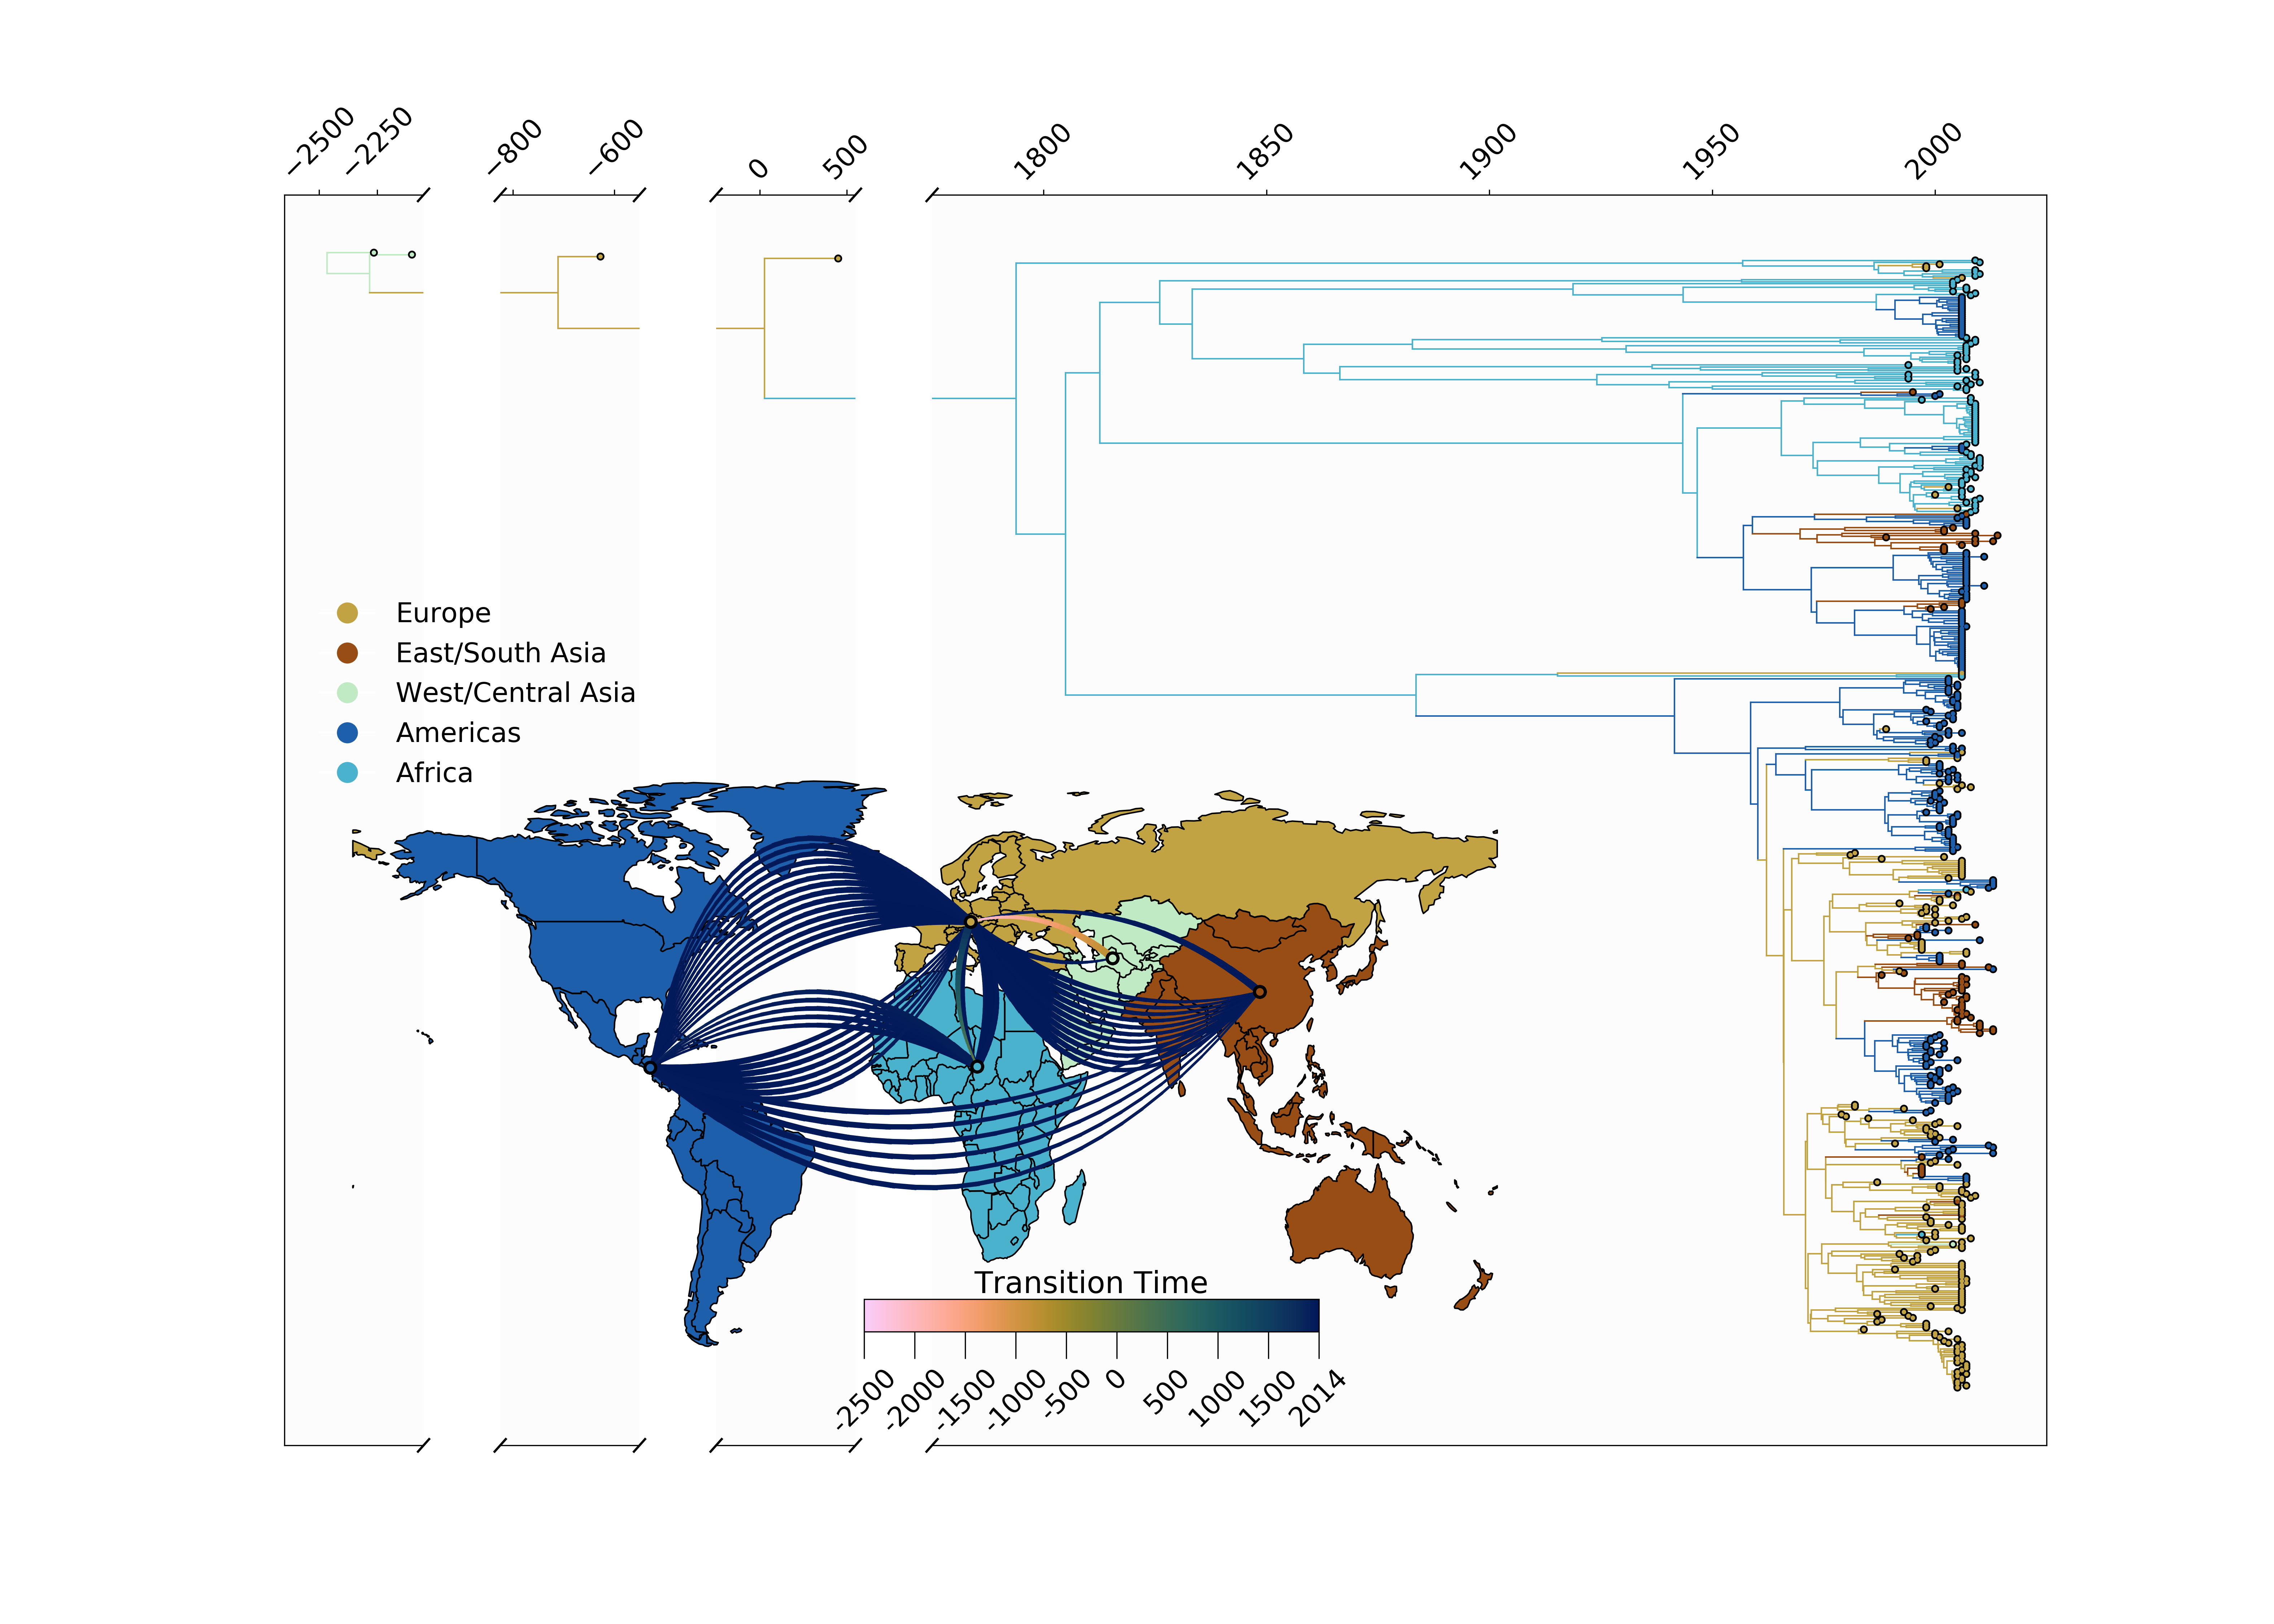
\includegraphics[width=.85\textwidth]{Figure4}
  \caption[HBV-A phylogeography]{Spatio-temporal transmission dynamics of \gls{hbv}-A. Time-scaled maximum clade credibility tree representing the spatio-temporal history of \gls{hbv} genotype A. The time of origin is inferred to be at 2504 BCE. Tips and branches are colored according to inferred location. Breaks in the time axis represent long periods of time covered by individual branches. (inset) World map colored according to the geographic regions used for the discrete phylogeographic analysis. Each line represents an inferred transmission event between two regions (55 total). Line colors denote timing intervals of each introduction. Concave up lines represent west to east movement, concave down lines represent east to west movement, concave right lines represent north to south movement, and concave left lines represent south to north movement. Europe shows the greatest number of outgoing introductions (29). West/Central Asia is the inferred root location of the tree, with one ancient transmission to Europe inferred to have taken place between 2243--876 BCE.}
  \label{fig:3-4}
\end{figure}

Using the same methods as for \gls{hbv}-A, we performed discrete phylogeographic inference for \gls{hbv}-D.
We estimate \gls{hbv}-D to have originated in East/South Asia around 1779 BCE, after which it rapidly spread to West/Central Asia.
We observe much more of \gls{hbv}-D's evolutionary history taking place in East/South Asia and West/Central Asia, with the former spawning introductions into Africa, the Americas, and Europe.
Most of the introductions into the Americas occur from Europe however, with Europe in turn being mostly seeded from East/South Asia (Fig.~\ref{fig:3-5}).
For \gls{hbv}-D, we observe a large impact of including the ancient sequences into our data set.
While we have shown that this leads to a large decrease in evolutionary rate, Fig.~\ref{fig:3-5} shows much older divergence times being estimated compared to a data set with only modern-day sequences (data not shown).
The \gls{tmrca} of the largest predominantly African lineage is estimated to be around 550 CE, with the oldest \gls{tmrca} of a mixed European/American clade estimated to be around 1100 CE.
We infer the \gls{mrca} of this clade to have existed within the Americas, however this timing does not correspond to any know human movement patterns, so we believe this inference to be an artifact of either heterogeneous sampling or the weak temporal signal of \gls{hbv}-D.
As with genotype A, individual clades show a strong local geographic structuring, with few individual location changes occurring except within the most recent 50 years.

We also performed similar phylogeographic reconstruction for \gls{hbv}-E, however without any ancient genomes, as none were publicly available (Fig.~\ref{fig:3-6}).
We estimated the \gls{tmrca} of \gls{hbv}-E to 1825 CE, with the introductions into Europe and the Americas estimated to have come directly from the African continent.
Given that nearly all European sequences in the tree appear as singletons, dating these introductions would be accompanied with much uncertainty.

\begin{figure}[ht]
  \centering
  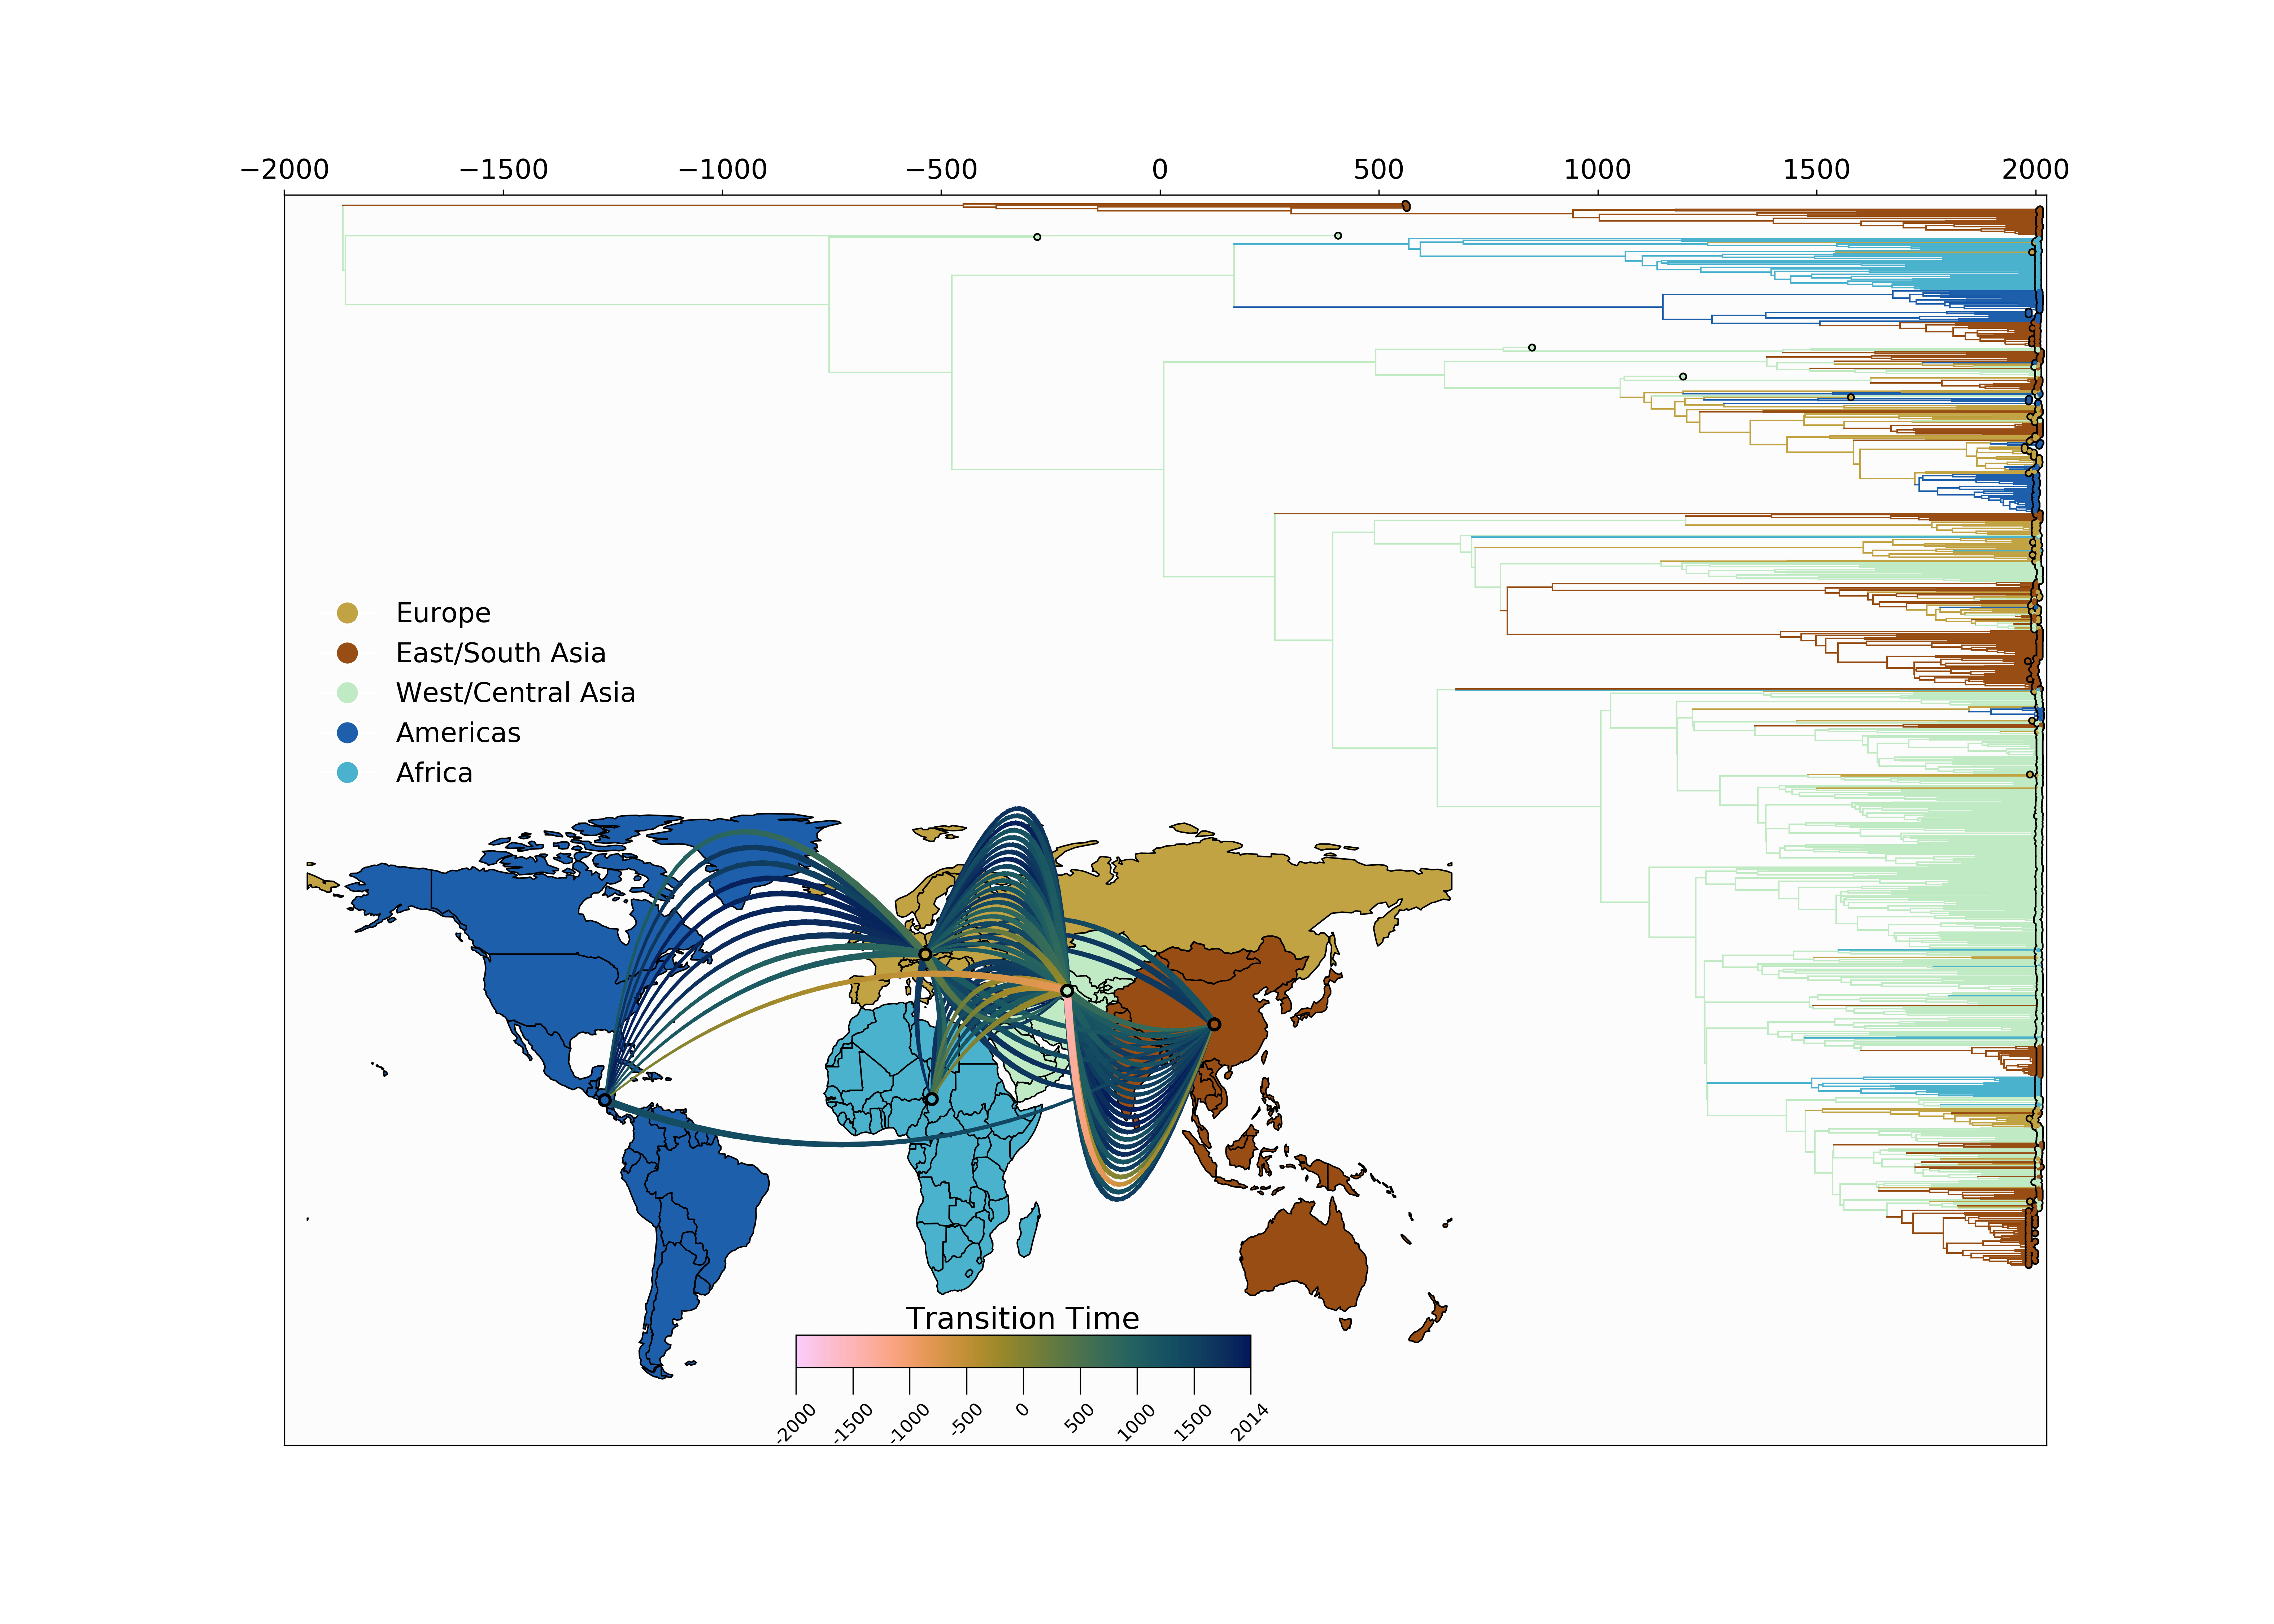
\includegraphics[width=.85\textwidth]{Figure5}
  \caption[HBV-D phylogeography]{Spatio-temporal transmission dynamics of \gls{hbv}-D. Time-scaled maximum clade credibility tree representing the evolutionary history of \gls{hbv} genotype D. The time of origin is inferred to be at 1779 BCE. Tips and branches are colored according to inferred locations. (inset) World map colored according to the geographic regions used for the discrete phylogeographic analysis. Each curved line represents an inferred transmission event between two regions (92 total). Line colors denote timing intervals of each introduction. Concave up lines represent west to east movement, concave down lines represent east to west movement, concave right lines represent north to south movement, and concave left lines represent south to north movement. West/Central Asia shows the greatest number of outgoing transmission events (55), as well as being the most likely location of the most recent common ancestor to sampled modern sequences.}
  \label{fig:3-5}
\end{figure}

\begin{figure}[ht]
  \centering
  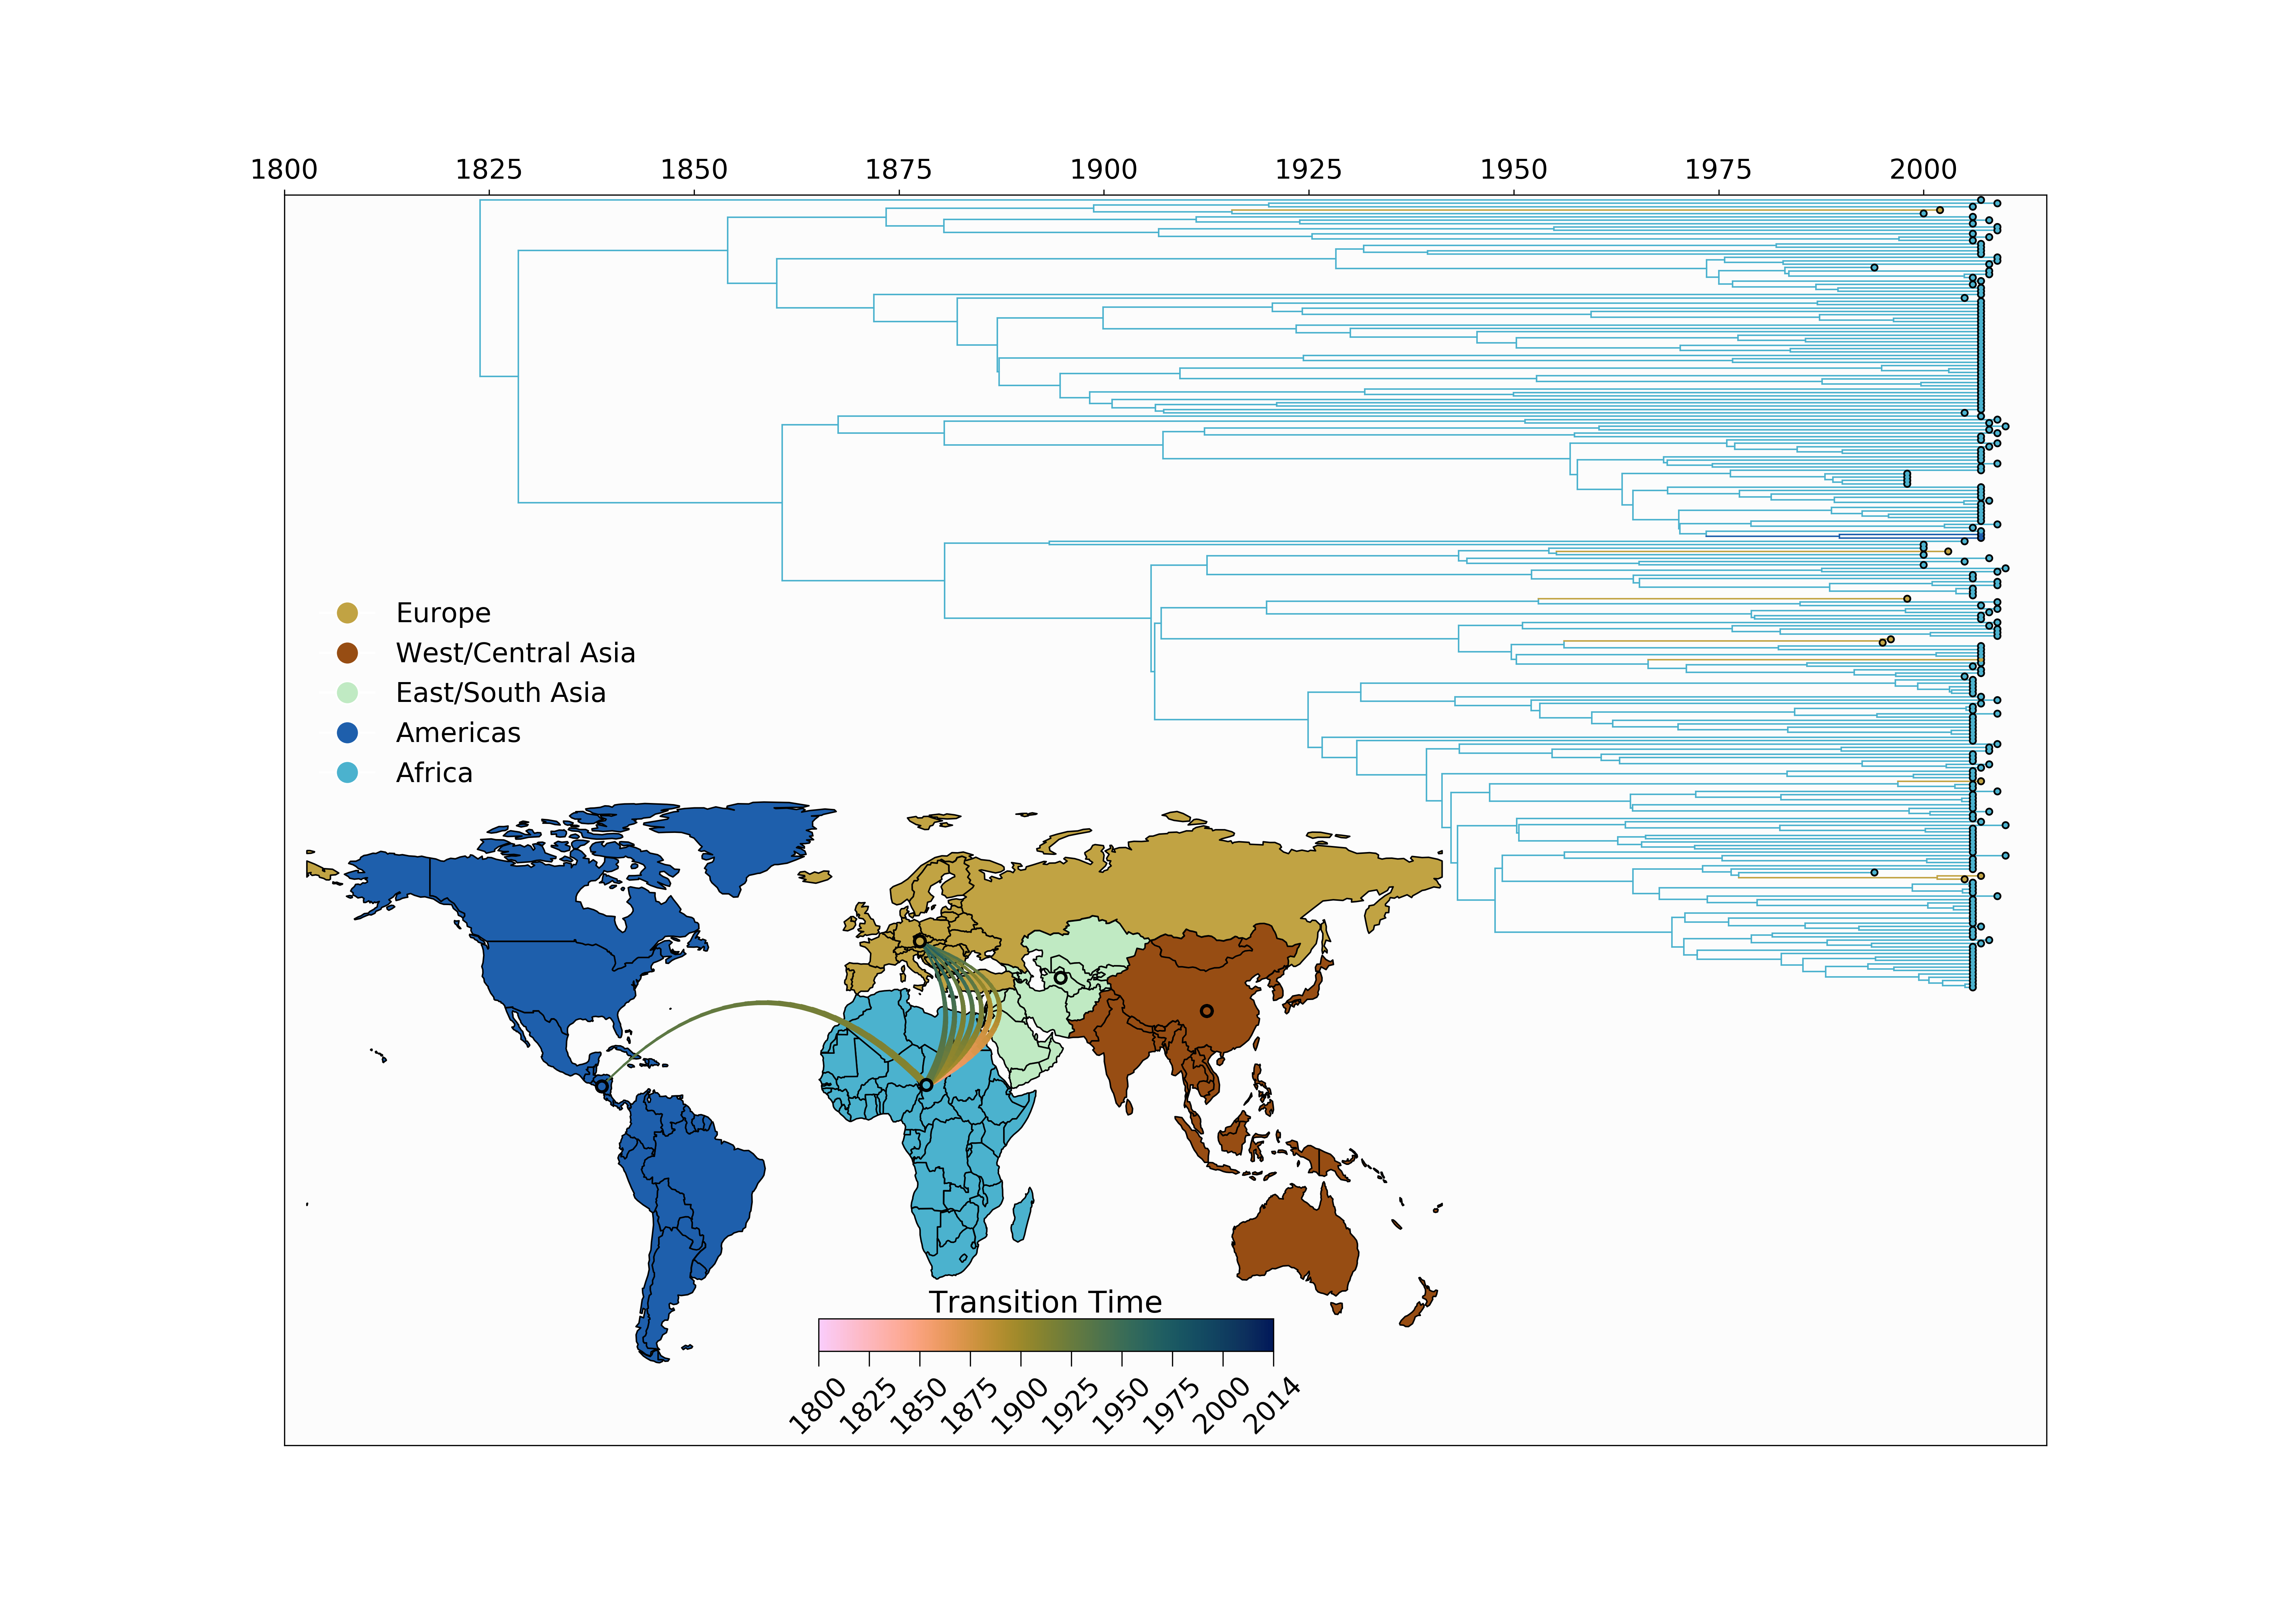
\includegraphics[width=.85\textwidth]{Figure6}
  \caption[HBV-E phylogeography]{Spatio-temporal transmission dynamics of \gls{hbv}-E. Time-scaled maximum clade credibility tree representing the evolutionary history of \gls{hbv} genotype E. The time of origin is inferred to be at 1824 CE. Tip and branches are colored  according to inferred location. (inset) World map colored according to the geographic regions used for the discrete phylogeographic analysis. Each counterclockwise arrow represents an inferred transmission event between two regions. Arrow colors denote timing intervals of each introduction. All migration events (8 total) are inferred to have originated in Africa; Europe was the destination of seven migrations, and the Americas were the destination of one.}
  \label{fig:3-6}
\end{figure}

We summarized the strongest supported rates of discrete location transitions between pairs of regions for each dataset (Fig.~\ref{fig:3-7}).
For \gls{hbv}-A, we find very strong Bayes factor support \citep{kass1995bayes} for movements from Europe to East/South Asia and the Americas, as well as strong support for movements from the Americas and Africa to Europe.
For \gls{hbv}-D, we observe very strong support for outgoing movements from West/Central Asia to Europe, Africa and East/South Asia.
We also find very strong support for outgoing movements from Europe to East/South Asia, West/Central Asia and the Americas.
Finally, for \gls{hbv}-E, we only find very strong support for movements from Africa into Europe and strong support for movements from Africa to the Americas.
For each genotype, we estimated Markov jump counts to quantify total geographic transitions.
We estimated 62 [95\% HPD: 51--72] transitions in the evolutionary history of \gls{hbv}-A, 92 [95\% HPD: 85--100] transitions in the evolutionary history of \gls{hbv}-D, and 8 [95\% HPD: 8--10] transitions in the evolutionary history of \gls{hbv}-E.

\begin{figure}[ht]
  \centering
  \includegraphics[width=.85\textwidth]{Figure7}
  \caption[Bayes factor support for HBV migrations]{Bayes factor support for \gls{hbv}'s geographic transitions. Networks representing posterior support for migrations between geographic regions as determined by \gls{bssvs} analysis. Inferred migrations are represented as curved lines. Bayes factors are represented by color intensity; darker lines depict higher Bayes factors, therefore higher posterior support. Direction of movement is represented by anticlockwise curvature of each line. In \gls{hbv}-A, we estimate strongly supported migrations out of Europe to all other regions, as well as high support for inferred migrations into Europe from Africa and the Americas. In \gls{hbv}-D, we observe well-supported migration history from Africa to Europe, and from Europe to the Americas and Asia. Finally, in \gls{hbv}-E, we observe very strong support for migration from Africa to Europe, as well as relatively high support for migration from Africa to the Americas.}
  \label{fig:3-7}
\end{figure}

\section{Discussion and Conclusion}
Human mobility exerts an immense pressure on the infectious disease profile and public health landscape of countries who receive significant numbers of immigrants \citep{thijssen2019mass}.
The prevalence and diversity of \gls{hbv} is disproportionately affected by immigration when compared with other bloodborne viruses such as \gls{hiv} and \gls{hcv}.
A recent large study showed that the frequency of \gls{hbv} infection in immigrants in parts of Europe is three times greater than for \gls{hiv} and four times greater than for \gls{hcv} \citep{gonzalez2020overt}.
Specific virological characteristics of \gls{hbv} such as a long window of infectiousness, possibilities of occult infection promoted by mutations \citep{pronier2020contribution,olusola2021profiles,raimondo2019update}, and undetectable levels of genome amplification without antigen production have raised concerns about cryptic movement of specific \gls{hbv} genotypes from countries of high endemicity to those of low endemicity \citep{azarkar2019epidemiology,zhu2016genetic,bedi2021occult}.
Systemic inequities in access to health services faced by immigrants in higher income countries \citep{smith2018migrant} compound with these virological characteristics to impair the implementation of effective public health responses to \gls{hbv}.

Despite the significant public health burden of \gls{hbv} worldwide, there is limited insight into the evolutionary history of its different genotypes.
To the best of our knowledge, we present the most comprehensive investigation to date on the origins of \gls{hbv} genotypes A, D, and E, owing to the large number of full-length African \gls{hbv} genomes and broad spatiotemporal distribution of sequences we consider.
In this study, we focused on \gls{hbv} genotypes obtained from African immigrants in Belgium upon their arrival from 2005 to 2010, along with a broad selection of other publicly available sequences, both contemporary and ancient.
Almost $16\%$ of \gls{hbv} carriers from our study cohort showed co-infection with two other bloodborne viruses (\gls{hiv} and \gls{hcv}) which makes the design of antiviral therapies more complicated in destination countries \citep{arora2021complexities,torimiro2018rates}.
Three distinct genotypes were detected in immigrants from 15 African countries: \gls{hbv}-E ($50.4\%$), \gls{hbv}-A ($41.4\%$), and \gls{hbv}-D ($8.6\%$).
This finding agrees with previous reports of \gls{hbv} genotype diversity in sub-Saharan countries \citep{forbi2013disparate,andernach2009slave}.
The diversity of imported genotypes underscores the potential for changes in the epidemiological landscape of \gls{hbv} in recipient countries \citep{mina201715,aguilera2020gehep}.
The \gls{hbv}-A strains that we generated belong to the subgenotypes A1, A3, and quasi-subgenotypes A4, A5, and A7 which have already been isolated from African \gls{hbv} carriers living in different parts of the world \citep{andernach2009slave,kurbanov2005new,olinger2006phylogenetic,pourkarim2010novel}.
The recent discovery of novel subgenotype A8 from our study cohort highlights the lack of comprehensive information about \gls{hbv} in African immigrants in Belgium.

There is a well-documented association between \gls{hbv} genotype and clinical outcome; this relation is further documented for individual \gls{hbv} \gls{orf} mutations \citep{mina2015genomic,mina201715,liu2009associations,mello2014hepatitis,hou2019hcc-associated}.
These associations between genotype-specific mutations in circulating African strains and clinical severity have been demonstrated, for instance with particular medically important mutations being mostly detected in the core gene of \gls{hbv} strains isolated from patients with end stage liver diseases such as hepatocellular carcinoma (\gls{hcc}) \citep{amougou2019enrichment,mbamalu2021hepatitis,mak2020molecular}.
The association between A1762T, G1764A, and A1762T/G1764A, G1896A, and an increased risk of HCC has been previously shown \citep{wei2017association}.
High frequency of pre-core and core mutations detected in \gls{hbv}-E and \gls{hbv}-A in our study highlights the importance of investigating individual origins for \gls{hbv} cases, so that clinical interventions can be targeted appropriately.
Importantly, we identified clinically and para-clinically related mutations at \gls{orf} S, as previously described \citep{olusola2021profiles,mak2020molecular,lin2021hepatitis}.

Excepting their most ancient origins, our results agree with the work of others, with \gls{hbv}-A demonstrating an African origin \citep{pourkarim2011molecular,pourkarim2010novel,pourkarim2010are,toye2021hepatitis}.
Our results underscore the African continent as the evolutionary cradle of \gls{hbv}-A diversification \citep{andernach2009slave,toye2021hepatitis}, and we date the proliferation and worldwide dispersal of this genotype to coincide with the transatlantic slave trade (1520s--1850s).
Similar to \gls{hbv}-A, we find the most ancient origins of \gls{hbv}-D to be in Central Asia, however we also infer the majority of its evolutionary history to remain in the region, with much later introductions into other global regions \citep{pourkarim2014molecularidentification}.
For both \gls{hbv}-A and \gls{hbv}-D, the location that we infer for the \gls{mrca} of the genotype corresponds to the location of the most ancient genomes that we included in the study.
As more ancient \gls{hbv}genomes from different locations and times become available, we propose incorporating them into a study such as ours to reduce the uncertainty of \gls{mrca} location and time inference.

Almost half of the \gls{hbv} strains that we generated in this study were classified as \gls{hbv}-E (Suppl.~Table~\ref{suptab:hbv-s2}).
This high proportion is supported by other studies from West African countries \citep{andernach2009slave,assih2018genetic}.
Because of low diversity along its entire length of genome, \gls{hbv}-E does not classify into subgenotypes \citep{forbi2010epidemic} which may point to \gls{hbv}-E having evolved more recently than other genotypes \citep{ingasia2020global}.
In this study dataset, three strains with recombination signature were detected (Suppl.~Fig.~\ref{supfig:hbv-s1}) as previously described \citep{mina2015genomic,pourkarim2010are,forbi2010epidemic,liu2020complete}.
Recombination can happen in over-populated locales with high prevalence of \gls{hbv}, mostly occurring in East Asia and Africa \citep{pourkarim2014molecularidentification,liu2020complete}.

We observed that \gls{hbv}-D was the fastest evolving among the genotypes we encountered.
\gls{hbv}-E is the most recently diverged genotype, however both its divergence and evolutionary rate estimates have large 95\% highest posterior density intervals, indicating that these estimates must be cautiously interpreted.
A plausible explanation for why we observe such wide confidence interval is that our \gls{hbv}-E dataset is considerably smaller than this (234 sequences), compared to the dataset sizes for the other genotypes (583 \gls{hbv}-A and 764 \gls{hbv}-D sequences).
The combination of fewer sequences and no available ancient genomes may combine to provide more uncertainty in the evolutionary rate estimate.
As future ancient \gls{hbv}-E genomes are sequenced, their addition to studies like this may add certainty to future analyses that may help validate our inferred \gls{tmrca} estimate.

There is recent evidence that \gls{hbv} has limited temporal signal warranting temporal and evolutionary estimation not reliable, particularly for very long timeframes, with the risk of underestimating when the \gls{mrca} of each genotype diverged from the ancestral \gls{hbv} lineage \citep{ross2018paradox}.
To avoid the inherent biases of estimating these measures for viruses that have an ancient time of divergence, we opted for analyzing each genotype separately.
Additionally, we include ancient \gls{hbv} genomes when possible to provide increased temporal signal in our dataset, thus making the estimation of evolutionary rate and \gls{tmrca} more reliable.
A recent study by \citet{kocher2021ten} performed similar temporal phylogenetic analysis of \gls{hbv} and found \gls{mrca} estimates for each genotype different from ours by approximately a factor of two.
This discrepancy may be explained by their use of a epoch-based time-dependent rate model, while we use a relaxed clock model for each genotype that we consider.
Epoch-based time-dependent rate models require sufficient data to calibrate the time-dependent rate phenomenon.
As we include only four \gls{hbv}-A and five \gls{hbv}-D ancient genomes in our genotype-split analysis, we find a relaxed clock model to be a more appropriate model for our datasets.
Additionally, differences may arise as a result of our analysis of each \gls{hbv} genotype separately, whereas \citet{kocher2021ten} consider the entire unified \gls{hbv} phylogeny.
We find different mean evolutionary rates for each genotype, suggesting that a single estimate for all genotypes may not fully capture the different evolutionary dynamics affecting each, not even when using a time-dependent rate model.

Rather than employing each individual country as a different location for our discrete phylogeographic reconstruction, we have opted to perform these analyses on the regional level in order to deal with sampling bias among the different countries in our data sets.
Our choice of continental groups for discrete phylogeographic reconstruction serves two purposes simultaneously.
First, by reducing from 54 countries present between our three datasets to five continental regions we are able to significantly reduce the otherwise computationally infeasible reconstruction to one in which we are able to accumulate sufficient sampling from the posterior distribution to make significant inferences---an end that would not be possible with such a large and sparse sampling of countries.
Secondly, because our phylogenetic reconstructions of the \gls{hbv} genotypes range from hundreds to thousands of years we find modern political designations to be unsatisfactory designations to describe historical patterns of viral evolution and spread, by keying our analysis to geographic regions we find that our results have increased interpretability in a historical context.
Unfortunately, to maintain consistent geographic subdivisions across datasets there remains significant heterogeneity in the number of sequences between regions for some analyses.
Phylogeographic inference using structured coalescent models \citep{maio2015new,muller2018mascot} offers a potential solution to deal with sampling bias, at the expense of much increased computational demands, however we have instead opted to use continent-level analysis here to reduce computational complexity \citep{hong2020search}.

This study highlights the importance of genotype-aware treatment of \gls{hbv} interventions, particularly in the case of individuals who have recently migrated from regions where \gls{hbv} diversity is high.
Because \gls{hbv} genotype and specific mutational profile can have a significant impact on clinical outcomes, we find it imperative that these characteristics be taken into account so that individuals receive appropriate clinical and public health support for their infecting \gls{hbv} genotype, and so that local diversity of \gls{hbv} is well characterized so that policymakers and public health institutions can create the most effective intervention strategies possible.
We believe this effort can be significantly assisted by both genetic analyses for individual level interventions, and by large-scale phylogenetic and phylogeographic analyses to inform population level interventions that can lessen the overall burden of hepatitis B.


\section*{Acknowledgements}
BIP and GB acknowledge support from the Internal Funds KU Leuven (Grant No. C14/18/094).
GB acknowledges support from the Research Foundation--Flanders (``Fonds voor Wetenschappelijk Onderzoek--Vlaanderen,'' G0E1420N, G098321N).
PL acknowledges support from the Research Foundation--Flanders (``Fonds voor Wetenschappelijk Onderzoek--Vlaanderen,'' G0D5117N, G0B9317N, G051322N).
The opinions expressed in this article are those of the authors and do not reflect the view of the National Institutes of Health, the Department of Health and Human Services, or the United States government.


%%%%%%%%%%%%%%%%%%%%%%%%%%%%%%%%%%%%%%%%%%%%%%%%%%
% Keep the following \cleardoublepage at the end of this file, 
% otherwise \includeonly includes empty pages.
\cleardoublepage

% vim: tw=70 nocindent expandtab foldmethod=marker foldmarker={{{}{,}{}}}
